\begin{frame}[t]{Otros comandos útiles}
    \begin{comando}
        git rm
    \end{comando}

    \only<2->{
        \begin{block}{}
            Permite borrar un archivo y marcarlo como \textit{preparado}. La sintaxis es \texttt{git rm [archivo]}
        \end{block}
    }

    \vspace{2em}

    \begin{comando}
        git mv
    \end{comando}

    \only<3->{
        \begin{block}{}
            Permite mover/renombrar un archivo y marcarlo como \textit{preparado}. La sintaxis es \texttt{git mv [archivo] [nuevo nombre/ubicación]}
        \end{block}
    }
\end{frame}

\begin{frame}[t]{Inspeccionando los cambios}
    \begin{comando}
        git diff
    \end{comando}

    \pause
    \begin{block}{}
        Muchas veces es conveniente ver cuales son los cambios realizados antes de marcarlos como \textit{preparados}.

        Para esto tenemos el comando \texttt{git diff}, que muestra las diferencias entre lo que hay en
        tu directorio de trabajo con lo que hay en tu área de preparación.

        \vspace{1em}

        Si en cambio, queremos ver los cambios que preparamos y que irán en la próxima confirmación, podemos usar \texttt{git diff --staged}.
    \end{block}

    \pause
    \begin{ejercicio}{Ejercicio}
        Modificar un archivo de algún repo de la clase pasada y ejecutar \texttt{git diff}
    \end{ejercicio}
\end{frame}

\begin{frame}[t]{Viendo la historia de los commits}
    \begin{comando}
        git log
    \end{comando}

    \pause
    \begin{block}{}
        Después de haber hecho varios \textit{commits}, o si acabamos de clonar un repositorio
        de internet, puede que querramos ver el historial de commits para ver cuales
        fueron las modificaciones que se hicieron. Esto se puede lograr utilizando el
        comando \texttt{git log}.
    \end{block}

    \pause
    \begin{ejercicio}{Ejercicio}
        Ejecutar \texttt{git log} en algún repo de la clase pasada.
    \end{ejercicio}
\end{frame}

\begin{frame}[t]{Ramificaciones en Git}

    % Git es distribuido

    Una rama en Git representa una linea independiente de desarrollo.
    Al crear nuevas ramas, podemos pensar que nuestro proyecto se diverge en dos distintos:
    los cambios que hagamos en uno no impactan al otro.

    \pause
    \vspace{0.5em}
    Un ejemplo visual:

    \begin{figure}[ht]
        \begin{center}
            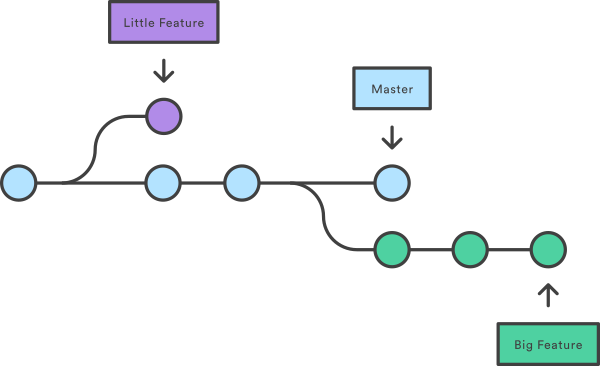
\includegraphics[height=1.5in]{images/branch.png}
        \end{center}
    \end{figure}

    % \only<3-3>{
    %     \begin{figure}[ht]
    %         \begin{center}
    %             \includegraphics[height=1.5in]{images/branch-1.png}
    %         \end{center}
    %         \caption{La rama ``master'' apunta al commit \textit{f30ab}}
    %     \end{figure}
    % }
    %
    % \only<4-4>{
    %     \begin{figure}[ht]
    %         \begin{center}
    %             \includegraphics[height=1.5in]{images/branch-2.png}
    %         \end{center}
    %         \caption{Creamos una nueva rama llamada ``testing''}
    %     \end{figure}
    % }


    % Ademas de tener ramas locales, podemos tenemos ramas remotas, que referencian al estado de ramas en tus repositorios remotos.
    % Si por ejemplo quisieramos saltar a la rama ``master'' en el repositorio remoto ``origin'' podríamos utilizar el comando \texttt{git checkout origin/master}.
    %
    % \vspace{1em}
    %
    % Nuestras ramas locales no sincronizan automaticamente con los repositorios remotos. Por esta razón, si tenemos una rama llamada ``master'' de forma local que
    % apunta a la rama remota ``origin/master'' podemos actualizarla parandonos en ``master'' y ejecutando \texttt{git pull origin master}.
    %
    % \vspace{1em}
    %
    % De forma análoga, si queremos publicar cambios locales aun repositorio remoto, tenemos el comando \texttt{git push}. Si estamos parados en la rama ``master'':
    % \texttt{git push origin master}.

\end{frame}

\begin{frame}[t]{Creando ramas}
    \begin{comando}
        git branch
    \end{comando}

    \pause
    \begin{block}{}
        Para crear una rama nueva, podemos ejecutar \texttt{git branch [nombre de la rama]}.

        Notese que este comando no nos mueve a la nueva rama, sólo la crea.
    \end{block}

    \pause
    \begin{ejercicio}{Ejercicio}
        Crear una rama llamada ``prueba'' en algún repo de la clase pasada.
    \end{ejercicio}

\end{frame}

\begin{frame}[t]{Cambiando de rama}
    \begin{comando}
        git checkout
    \end{comando}

    \pause
    \begin{block}{}
        Para cambiar de rama, podemos ejecutar \texttt{git checkout [nombre de la rama]}.
    \end{block}

    \pause
    \vspace{0.5em}
    Un ejemplo visual:
    \only<3-3>{
        \begin{figure}[ht]
            \begin{center}
                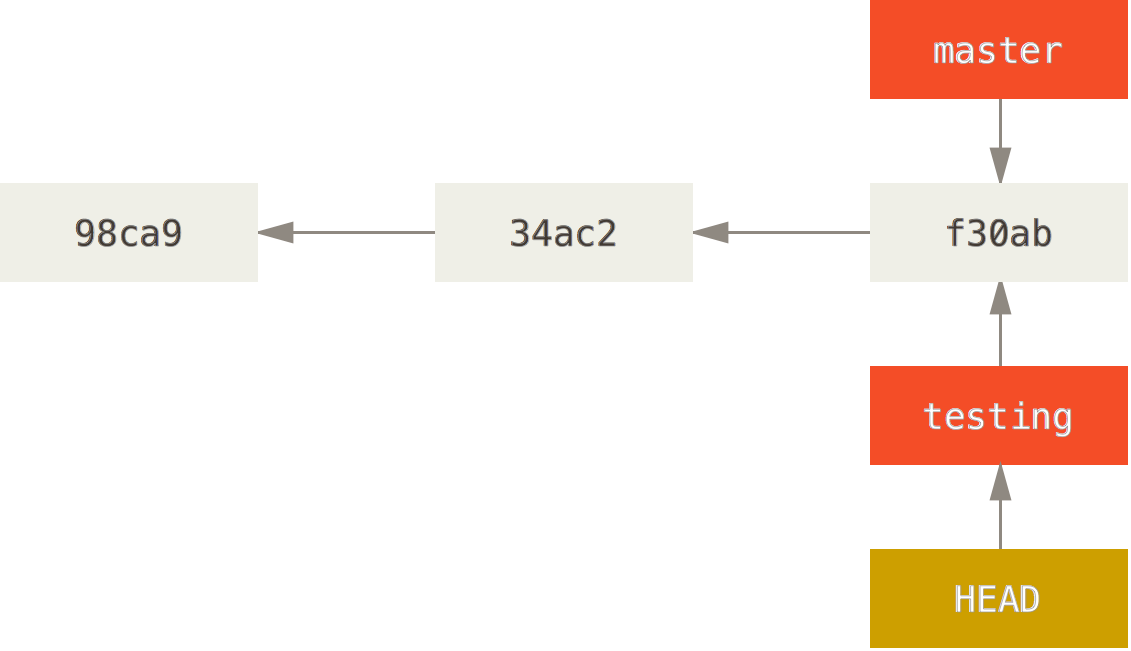
\includegraphics[height=1.3in]{images/head-to-testing.png}
            \end{center}
            \caption{Acá cambiamos a la rama ``testing'' ejecutando \texttt{git checkout testing}}
        \end{figure}
    }

    \only<4-4>{
        \begin{figure}[ht]
            \begin{center}
                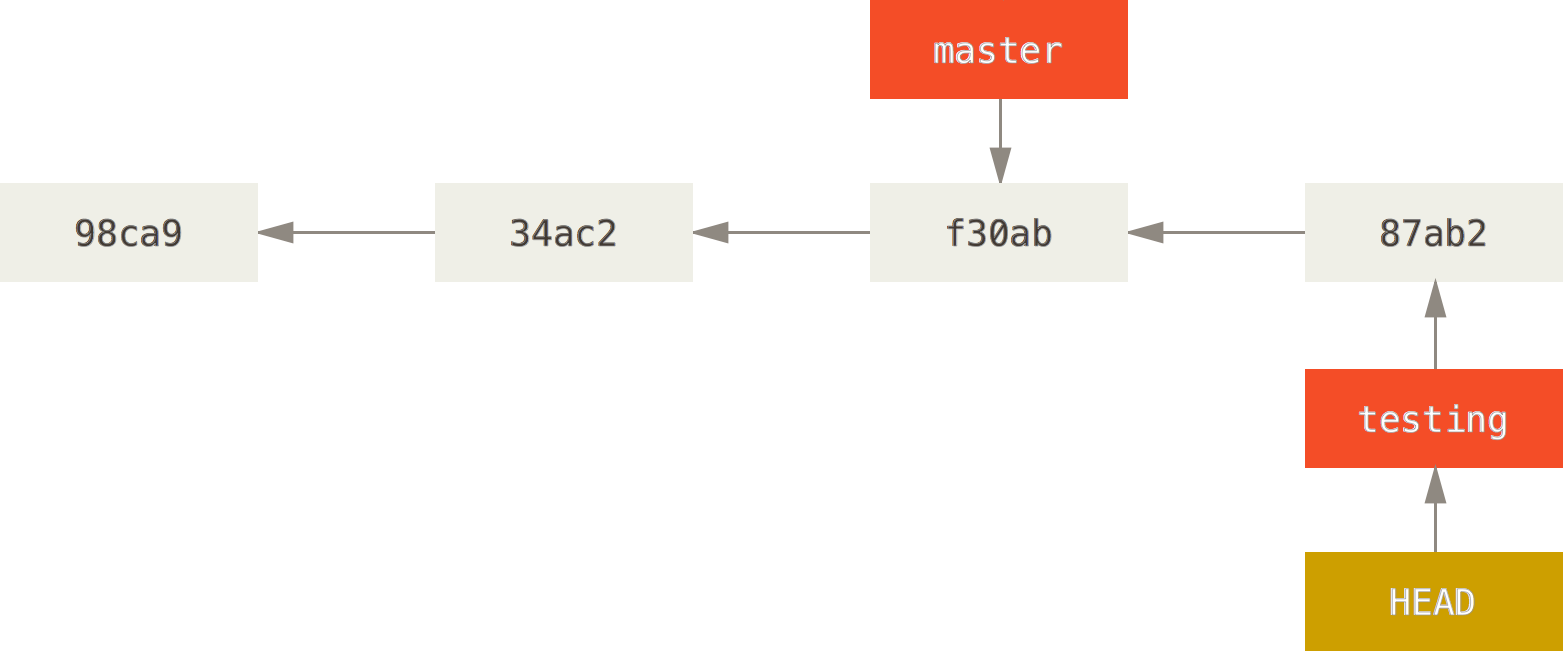
\includegraphics[height=1.3in]{images/advance-testing.png}
            \end{center}
            \caption{Y los siguientes commits serán agregados a la rama ``testing''}
        \end{figure}
    }

\end{frame}

\begin{frame}[t]{Fusionando ramas}
    \begin{comando}
        git merge
    \end{comando}

    \pause
    \only<2-2>{
        \begin{block}{}
            Nos permite fusionar las historias de 2 ramas distintas (podría haber conflictos).

            La sintaxis es: \texttt{git merge [nombre de la rama a fusionar]}.

            \textbf{Importante:} este comando fusiona la rama que le decimos
            \textbf{en la rama en la que estemos parados}.
        \end{block}
    }

    \pause
    Un ejemplo visual:
    \only<3-3> {
    	\begin{figure}[ht]
    		\begin{center}
    			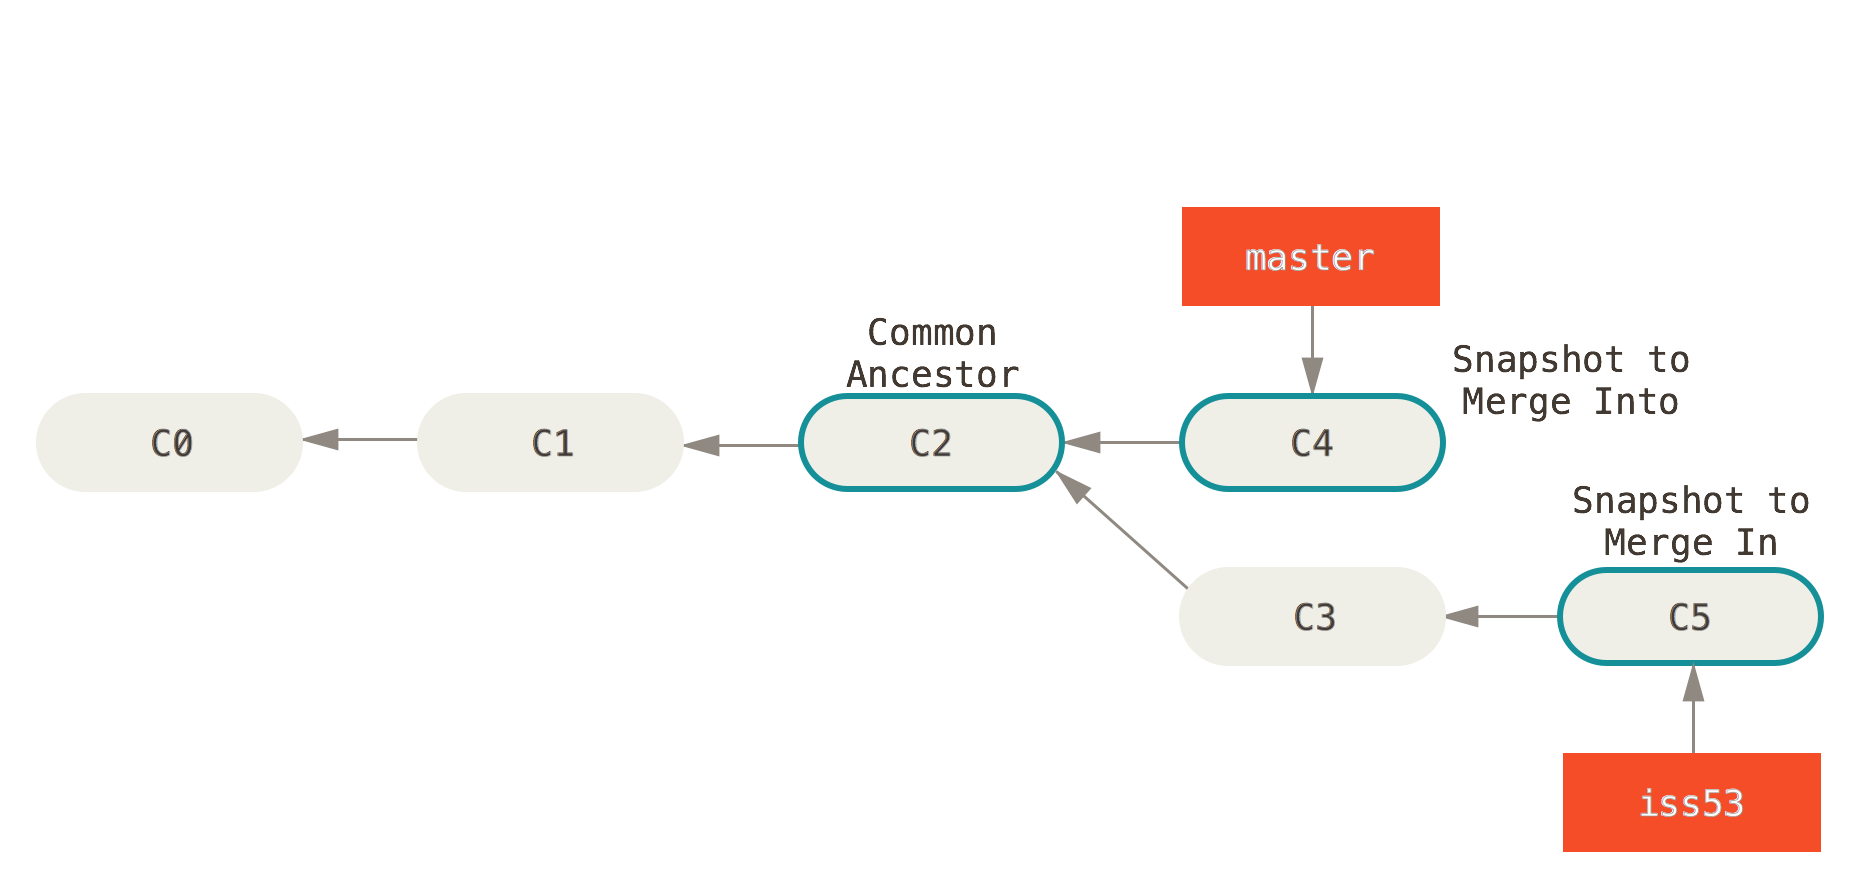
\includegraphics[height=1.5in]{images/merge-1.png}
    		\end{center}
    		\caption{Antes del merge}
    	\end{figure}
    }
    \only<4-4> {
        \begin{figure}[ht]
    		\begin{center}
    			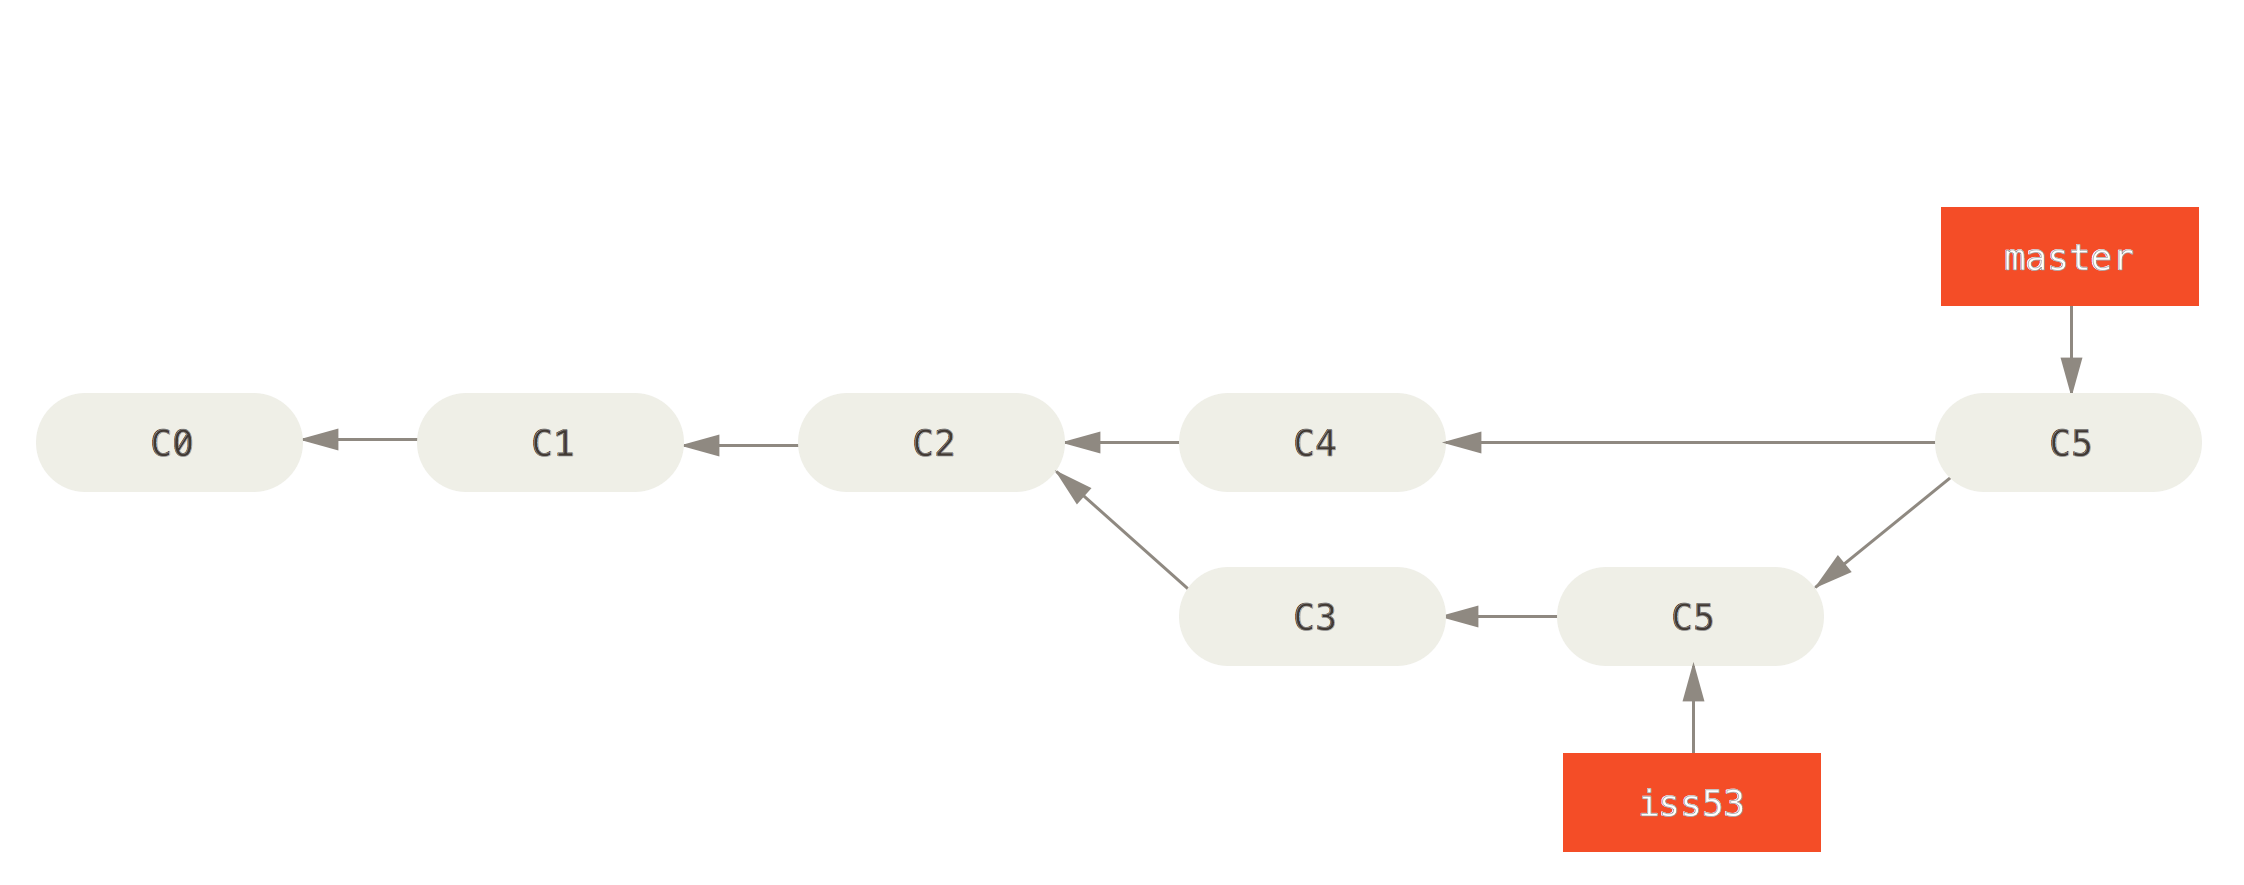
\includegraphics[height=1.5in]{images/merge-2.png}
    		\end{center}
    		\caption{Después de pararnos en la rama ``master'' (\texttt{git checkout master}) y haber fusionado la rama ``iss53'' \texttt{git merge iss53}}
    	\end{figure}
    }
\end{frame}

\begin{frame}[t]{A practicar!}
    Ejercicio largo de branches (no interactivo)

\end{frame}

\begin{frame}[t]{Revirtiendo cambios}
    \begin{comando}
        git commit --amend
    \end{comando}

    \only<2->{
        \begin{block}{}
            Podemos usarlo para arreglar por ejemplo el mensaje del último commit que hicimos: \texttt{git commit --amend -m [nuevo mensaje]}
        \end{block}
    }

    \vspace{2em}

    \begin{comando}
        git revert
    \end{comando}

    \only<3->{
        \begin{block}{}
            Permite \textit{revertir} exactamente los cambios introducidos por un commit. Buscamos el hash del commit en cuestión
            usando \texttt{git log}, y luego ejecutamos \texttt{git revert [hash]}.
        \end{block}
    }
\end{frame}

\begin{frame}[t]{Otro comando útil}
    \begin{comando}
        git stash
    \end{comando}

    \pause
    \begin{block}{}
        Al ejecutar \texttt{git stash}, guarda el estado actual de los archivos modificados que no están marcados como \textit{preparados} y nos deja el directorio limpio.

        \vspace{0.5em}

        Para volver a mostrar los cambios guardados ejecutamos \texttt{git stash pop}.
    \end{block}
\end{frame}

\begin{frame}[t]{Extras: Ignorando archivos}

    \begin{block}{El archivo .gitignore}
      Es común tener archivos generados automaticamente que no queremos agregar al repositorio. Por ejemplo, archivos compilados: .pdf, .exe, .log, .pyc, etc

      Sin embargo es bastante molesto verlos todo el tiempo al ejecutar \texttt{git status}.

      Para arreglar esto, podemos crear un archivo especial llamado \texttt{.gitignore} que le indica a Git que archivos ignorar por completo.
    \end{block}

    \pause
    \begin{resumen}{}
      Por ejemplo, para ignorar todos los archivos con extensión \textit{.pyc}:
      \begin{enumerate}
        \item Crear un archivo llamado \texttt{.gitignore} en el directorio principal del proyecto.
        \item Y adentro escribir: \textit{*.pyc}
      \end{enumerate}
      Más ejemplos de \texttt{.gitignore}: \url{https://github.com/github/gitignore}
    \end{resumen}


\end{frame}

\begin{frame}[t]{Extras: comandos}

    \begin{itemize}
        \item \texttt{git fetch [remote repository]}: para traer todos los datos de un repositorio remoto.
        \item \texttt{git reset}: para deshacer cambios, ya sea en el area de trabajo o en los commits.
        \item \texttt{git rebase [branch]}: aplica todos los commits que difieren entre un branch y el que estamos parados.
        \item \texttt{git blame [archivo]}: ?.
        \item \texttt{git bisect}: ?.
    \end{itemize}

\end{frame}

\begin{frame}[t]{Extras: servidores}

    \begin{figure}[ht]
        \begin{center}
            
\includegraphics[height=0.7in]{images/github.png}
        \end{center}
    \end{figure}

    \begin{figure}[ht]
        \begin{center}
            
\includegraphics[height=0.5in]{images/bitbucket.png}
        \end{center}
    \end{figure}

    \begin{figure}[ht]
        \begin{center}
            
\includegraphics[height=0.7in]{images/gitlab.png}
        \end{center}
    \end{figure}

\end{frame}

\begin{frame}[t]{Bibliografía}

    \begin{itemize}
        \item Git Community book, disponible online y en español: \url{https://git-scm.com/book/es/v2}
		\item \texttt{git help [command]} para ver la documentación de cualquier comando de Git.
		\item A visual Git reference: \url{http://marklodato.github.io/visual-git-guide/index-es.html}
		\item Try Git online: \url{https://try.github.io}
    \end{itemize}

\end{frame}
